\paragraph{Results.} Validation selected $\gamma=\SimGamma$ (the largest value in the grid) and a GP length scale of \SimLengthscale\,d. On the \SimNEvents\ Nominal test events (\SimNModeled\ modeled, \SimNWithheld\ withheld), H1 \SimHOneVerdict, H2 and H3 \SimHTwoVerdict. Table~\ref{tab:sim} lists every strategy in every scenario.

\paragraph{H1, identification speed: refuted.} P reached posterior $\geq0.95$ on the true class after a median of \SimTtiP\ and did so for \SimIdP\ of modeled events (Fig.~\ref{fig:tti}). It was faster than fixed cadence (which identified only \SimIdBzero), the auction baseline (median \SimTtiBone) and closed-world EIG (\SimTtiBthree; Holm $p$ \SimHolmBthree\ for each). It was not faster than classifier-entropy sampling B2, whose median was \SimTtiBtwo. The paired test favours P over B2 (Holm $p=\SimHolmBtwo$) only because B2 identified just \SimIdBtwo\ of events and unidentified events rank last. Pair by pair, P was slower in \SimSlowerBtwo\ of pairs and faster in \SimFasterBtwo. The preregistered criterion requires a shorter median, so H1 fails. P beats closed-world EIG here for an unflattering reason: under causality B3 greedily jumps to late, high-contrast epochs and uses only \SimObsAllBthree\ of its 5 measurements, against \SimObsAllP\ for P.

\begin{figure}[t]
\centering
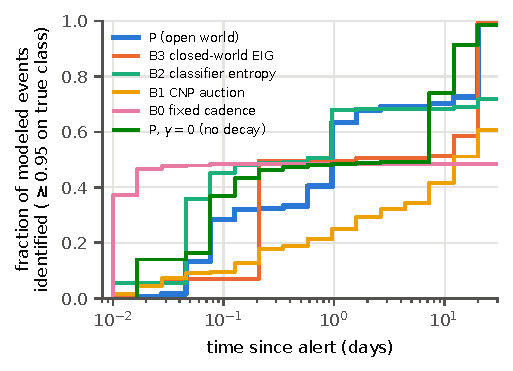
\includegraphics[width=\columnwidth]{generated/figures/fig1_tti.pdf}
\caption{H1. Cumulative fraction of modeled events whose posterior on the true class has reached 0.95, by time since alert (Nominal, test). B2 identifies the events it identifies earliest; P identifies almost all of them but later; closed-world EIG (B3) defers many identifications to the final epochs.}
\label{fig:tti}
\end{figure}

\paragraph{H2, irreversibility: supported, with caveats.} Removing the decay term reduced the information recovered about the true class's amplitude by \SimHtwoFast\ nats on fast classes and \SimHtwoSlow\ on the slow GRB afterglow, a difference of \SimHtwoEst\ \SimHtwoCI. The effect is carried by kilonovae (\SimDeltaKilonova) and, less, shock cooling (\SimDeltaShock); for the fastest class, the M-dwarf flare, the decay term \emph{lost} information (\SimDeltaFlare; Fig.~\ref{fig:decay}). It also reversed under model error, where the misspecified timescales mislead the urgency estimate (\SimHtwoModelErrorEst\ \SimHtwoModelErrorCI).

\begin{figure}[t]
\centering
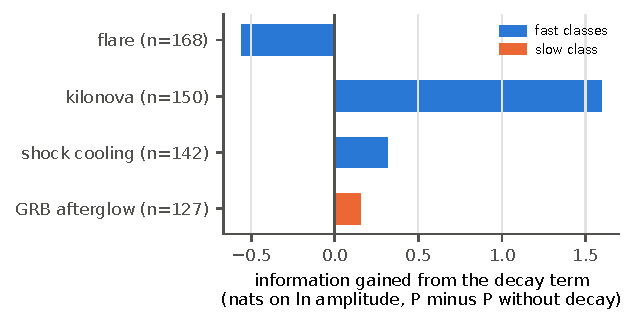
\includegraphics[width=\columnwidth]{generated/figures/fig2_decay.pdf}
\caption{H2. Per-class information about the true amplitude gained by the decay term (P minus P without it), Nominal test. Positive for kilonova and shock cooling, near zero for the slow class, negative for flares.}
\label{fig:decay}
\end{figure}

\paragraph{H3, open-world detection: supported.} At a 5\% false-alarm rate on modeled events, P's $P(h_0)$ detected \SimTprP\ of withheld events; thresholding the closed-world posterior entropy of B3 detected \SimTprBthree\ (difference \SimHthreeEst\ points, 95\% CI \SimHthreeCI; Fig.~\ref{fig:rocsim}). AUROCs were \SimAucP\ for $P(h_0)$ against \SimAucBthree\ (B3 entropy) and \SimAucBtwo\ (B2 entropy). Entropy computed on P's own measurements did no better (\SimAucPown), so the gain comes from the hypothesis, not from P's choice of measurements. Without $h_0$, closed-world EIG was confidently wrong on \SimCwWhBthreeAll\ of withheld events; P on \SimCwWhPAll, with no false ``unknown'' calls on modeled events (\SimFaP) and the same modeled accuracy as B3 (\SimAccModPAll). H3 held in all three scenarios, but model error is the predicted failure mode: P then called \SimFaPModelError\ of modeled events unknown and its modeled accuracy fell to \SimAccModPModelError\ (B3: \SimAccModBthreeModelError).

\begin{figure}[t]
\centering
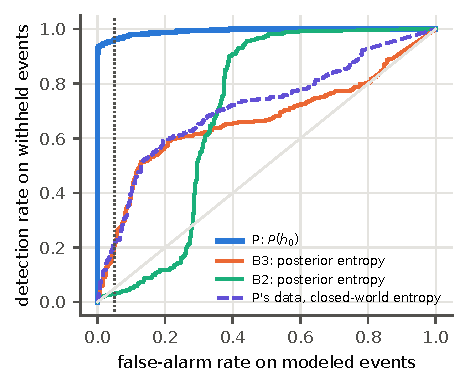
\includegraphics[width=\columnwidth]{generated/figures/fig3_roc_sim.pdf}
\caption{H3. ROC for separating withheld from modeled events (Nominal, test). Dotted line: the preregistered 5\% false-alarm operating point.}
\label{fig:rocsim}
\end{figure}

\paragraph{Ablations.} Removing the adequacy term changed nothing measurable: P$_{\beta=0}$ flagged \SimFlagNoAdeq\ of withheld events (P: \SimFlagP) with AUROC \SimAucAblNoAdeq\ (P: \SimAucAblP). Removing the decay term mattered: P$_{\gamma=0}$ took \SimObsAllNoDecay\ measurements instead of \SimObsAllP, flagged \SimFlagNoDecay, and was confidently wrong on \SimCwWhNoDecayAll\ of withheld events. In this setting the decay term's main effect on open-world detection is to stop the planner from spending its horizon too early, which gives $h_0$ enough data.

\begin{table*}[t]
\centering\scriptsize
\caption{Simulation test results (1000 events per scenario). Acc.\ mod.: accuracy on modeled events (\%); CW: confident-wrong rate (\%) on unmodeled (withheld) and modeled events; $\bar n_{\rm obs}$: measurements used of 5; log score: mean log probability of the true outcome (closed-world strategies cannot express ``withheld'' and are floored at $10^{-6}$).}
\label{tab:sim}
\begin{tabular}{llrrrrr}
\toprule
Scenario & Strategy & Acc.\ mod. & CW unmod. & CW mod. & $\bar n_{\rm obs}$ & log score \\
\midrule
Nominal & P (open world) & 100 & 6 & 0 & 4.2 & -0.19 \\
 & B3 closed-world EIG & 100 & 97 & 0 & 2.8 & -5.71 \\
 & B2 classifier entropy & 88 & 69 & 0 & 4.9 & -5.82 \\
 & B1 CNP auction & 80 & 75 & 0 & 3.2 & -5.92 \\
 & B0 fixed cadence & 79 & 1 & 0 & 5.0 & -5.92 \\
 & P, $\gamma=0$ (no decay) & 99 & 31 & 0 & 3.6 & -0.87 \\
 & P, $\beta=0$ (no adequacy) & 100 & 6 & 0 & 4.3 & -0.20 \\
\midrule
Crowding & P (open world) & 99 & 14 & 0 & 4.0 & -0.43 \\
 & B3 closed-world EIG & 100 & 94 & 0 & 3.0 & -5.82 \\
 & B2 classifier entropy & 94 & 80 & 0 & 4.8 & -5.88 \\
 & B1 CNP auction & 86 & 71 & 0 & 3.1 & -5.97 \\
 & B0 fixed cadence & 76 & 1 & 0 & 5.0 & -6.03 \\
 & P, $\gamma=0$ (no decay) & 100 & 31 & 0 & 3.4 & -0.96 \\
 & P, $\beta=0$ (no adequacy) & 99 & 14 & 0 & 4.1 & -0.43 \\
\midrule
Model error & P (open world) & 87 & 21 & 8 & 3.9 & -1.21 \\
 & B3 closed-world EIG & 99 & 96 & 1 & 2.9 & -6.11 \\
 & B2 classifier entropy & 81 & 29 & 4 & 5.0 & -6.32 \\
 & B1 CNP auction & 82 & 72 & 1 & 3.2 & -6.29 \\
 & B0 fixed cadence & 77 & 1 & 0 & 5.0 & -6.25 \\
 & P, $\gamma=0$ (no decay) & 93 & 26 & 6 & 3.4 & -1.32 \\
 & P, $\beta=0$ (no adequacy) & 86 & 21 & 8 & 3.9 & -1.21 \\
\bottomrule
\end{tabular}

\end{table*}
